\section{Evaluation}

\subsection{"SEE" Desktop}
In this section the desktop version of \enquote{\gls{see}} will be explained. 
In this evaluation the mobile version of \enquote{\gls{see}} will be compared with the desktop version.
Therefore, it is necessary to take a deeper look at the differences between those two versions.

\subsection{Aim and hypotheses}
The finished prototype of the mobile extension shall be evaluated. 
Therefor the system shall be compared on smartphones as well as desktop computers. 
Comparing these two use cases shall give insight on how much impact the constraints of mobile devices have on the usability and overall user experience.

The hypotheses of this thesis is that the mobile version of \enquote{\gls{see}} lacks slightly in usability compared to the desktop version.
This due to the constraints of the mobile device. 
A smartphone has far less screen space and also does not have a physical keyboard, which would allow many more shortcuts.
\subsection{Experiment set up}
The system shall be tested in two groups each starting with a different device. 
Each group does the test on both devices, but one group will start with the mobile application and the other one with the desktop application.
The participants will be assigned random to the groups.
The testers will have various tasks to test parameters such as understandability, learnability, operability and attractiveness. 
Afterwards the users will get a survey in English or German to document their impressions.
The survey shall also conclude differences between screen sizes and Android versions. 

To not exhaust the testers too much the experiment shall not take longer than one hour. 
This also ensures that there is not to little variance due to exhaustion.
Each participant might have a different concentration span, but this shall not be the focus of this experiment. 

\begin{figure}[htb]
    \centering
    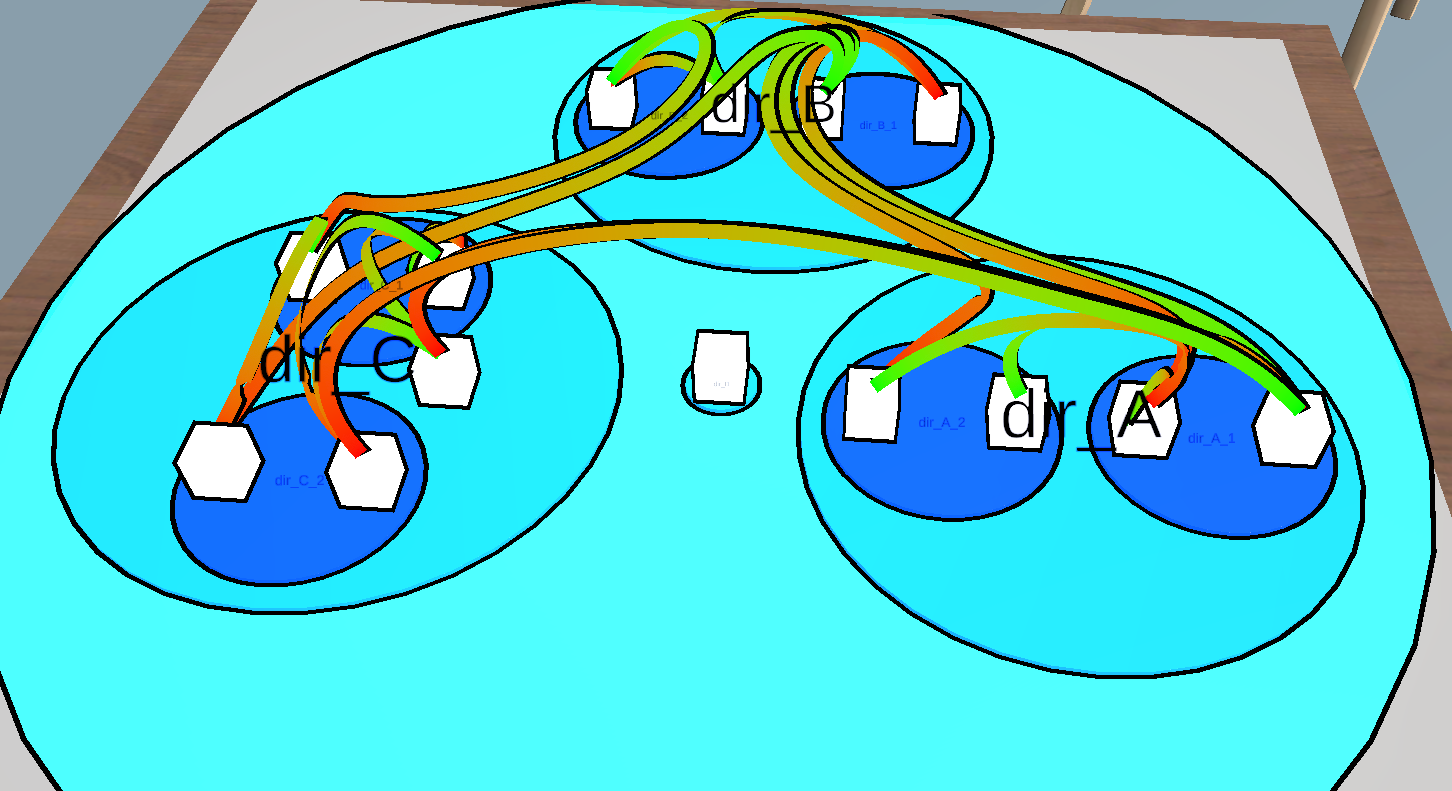
\includegraphics[width=1\textwidth]{Evaluation/img/city_1.png}
    \caption{The first \enquote{\gls{city}} for the user study}\label{fig:city1}
\end{figure}

\begin{figure}[htb]
    \centering
    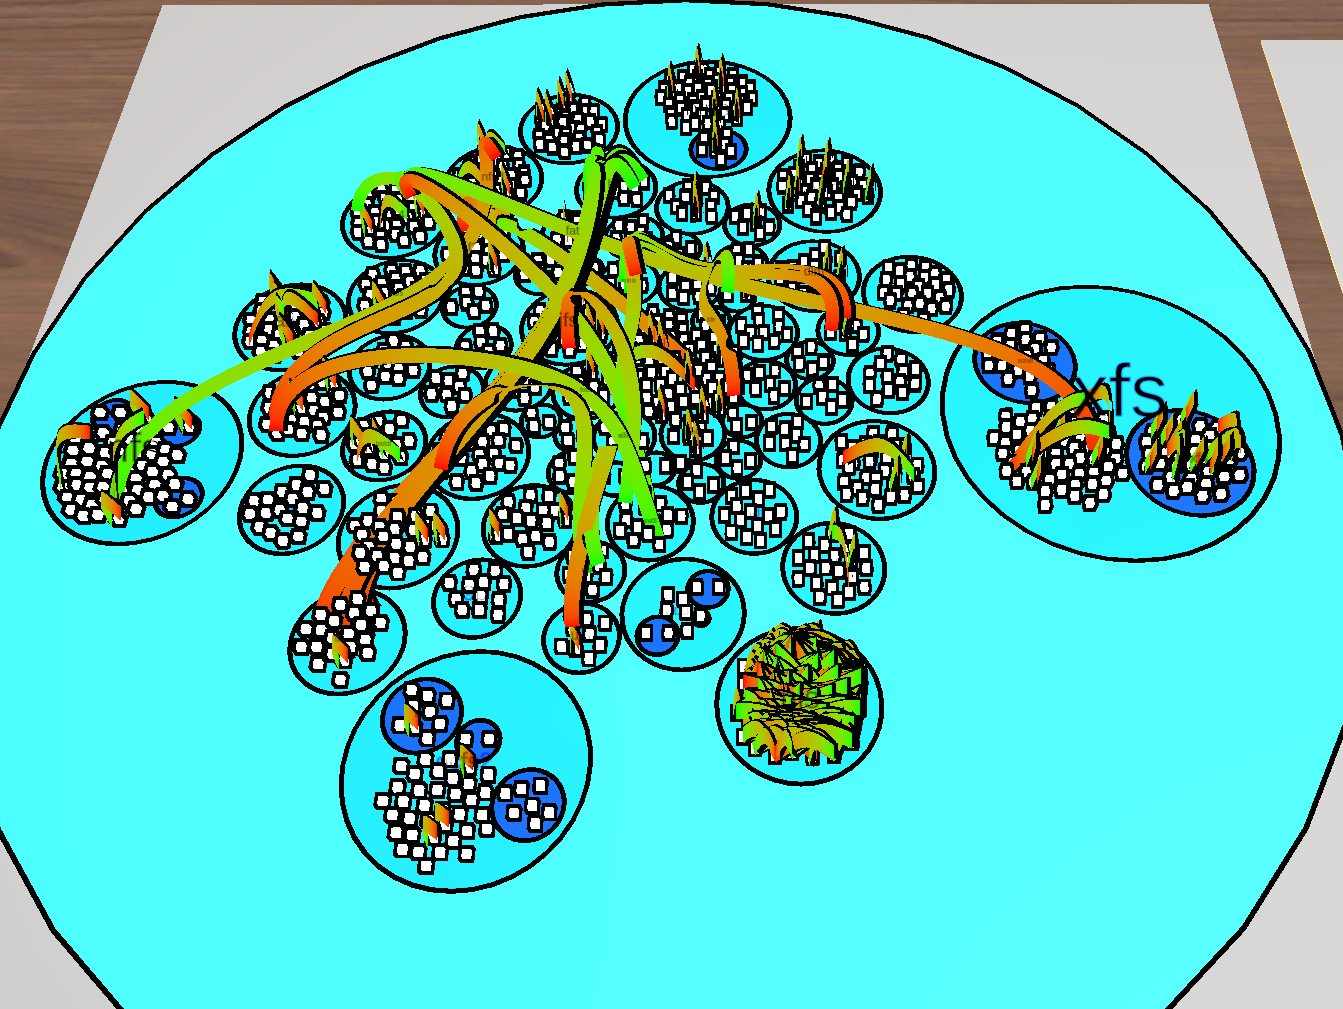
\includegraphics[width=1\textwidth]{Evaluation/img/city_2.png}
    \caption{The second \enquote{\gls{city}} for the user study}\label{fig:city2}
\end{figure}

\subsection{Realization}
\subsection{Survey tool}
\subsubsection{Pilot study}
In a first test the pilot study was executed with one tester. 
Afterwards the study was discussed and checked for errors. 
It stood out that the example \enquote{\gls{city}} of task one was too different to the one in the second task.
Therefore, the \enquote{\gls{city}} of the first task was exchanged with a larger and better comparable one.
Further on a \enquote{\gls{city}} with 1288 nodes (see figure \ref{fig:city3}) as well as one with 1464 nodes (see figure \ref{fig:city2}) will be used.

Also, the tasks were not comparable because they differed in the types of interactions they used.
In one task the user was asked to rename a node and in the other one the user shall add four nodes.
For renaming a node the user has to use a keyboard which does not make it comparable to just click and add nodes in the second task.


\begin{figure}[htb]
    \centering
    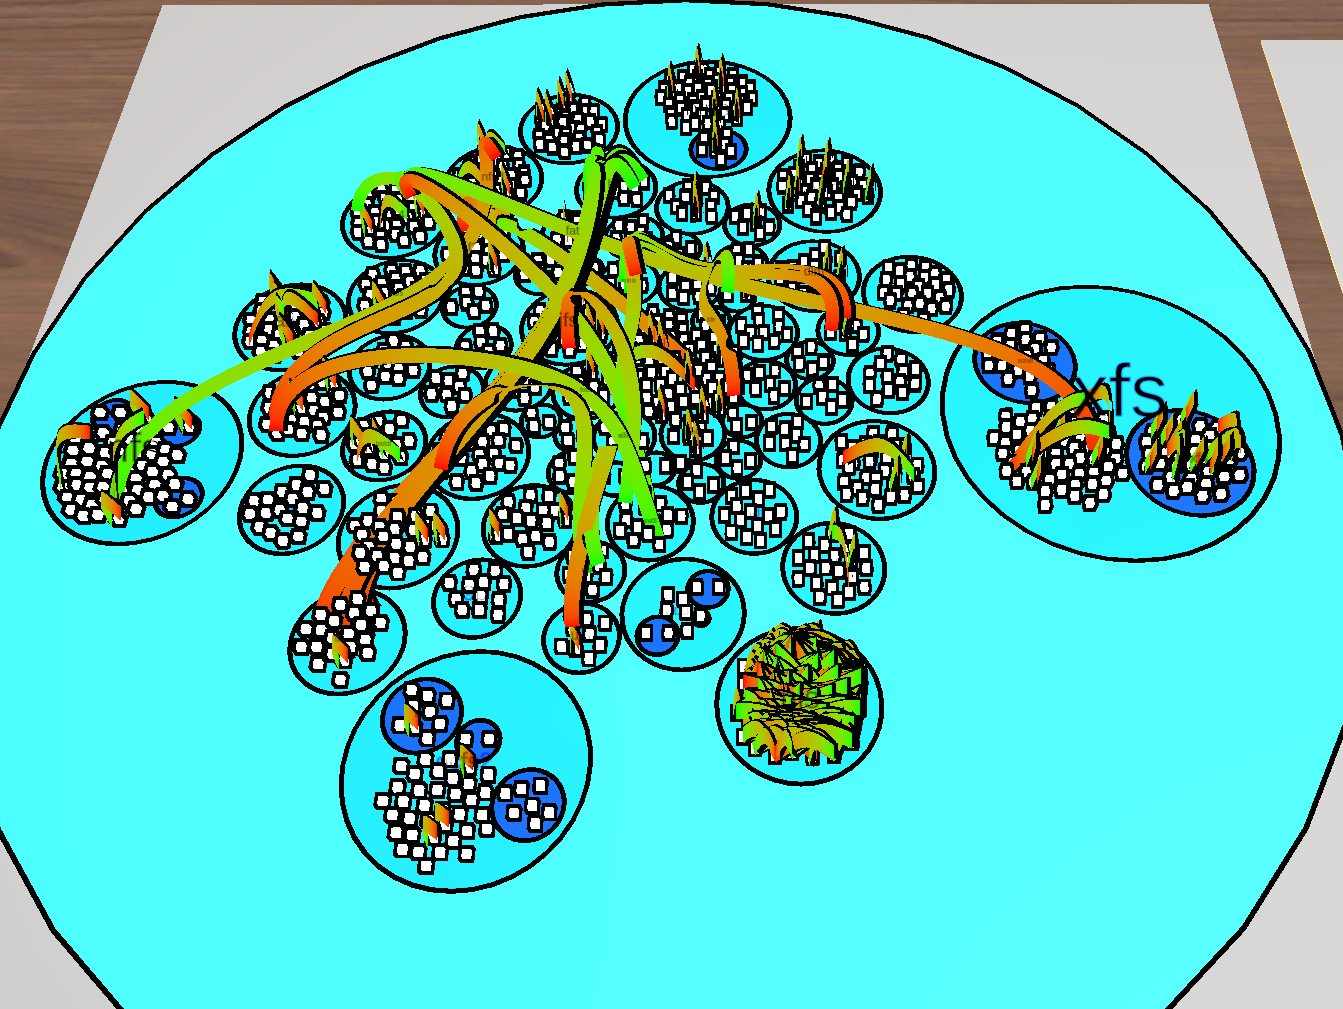
\includegraphics[width=1\textwidth]{Evaluation/img/city_3.png}
    \caption{The third \enquote{\gls{city}} for the user study}\label{fig:city3}
\end{figure}

\begin{figure}[htb]
    \centering
    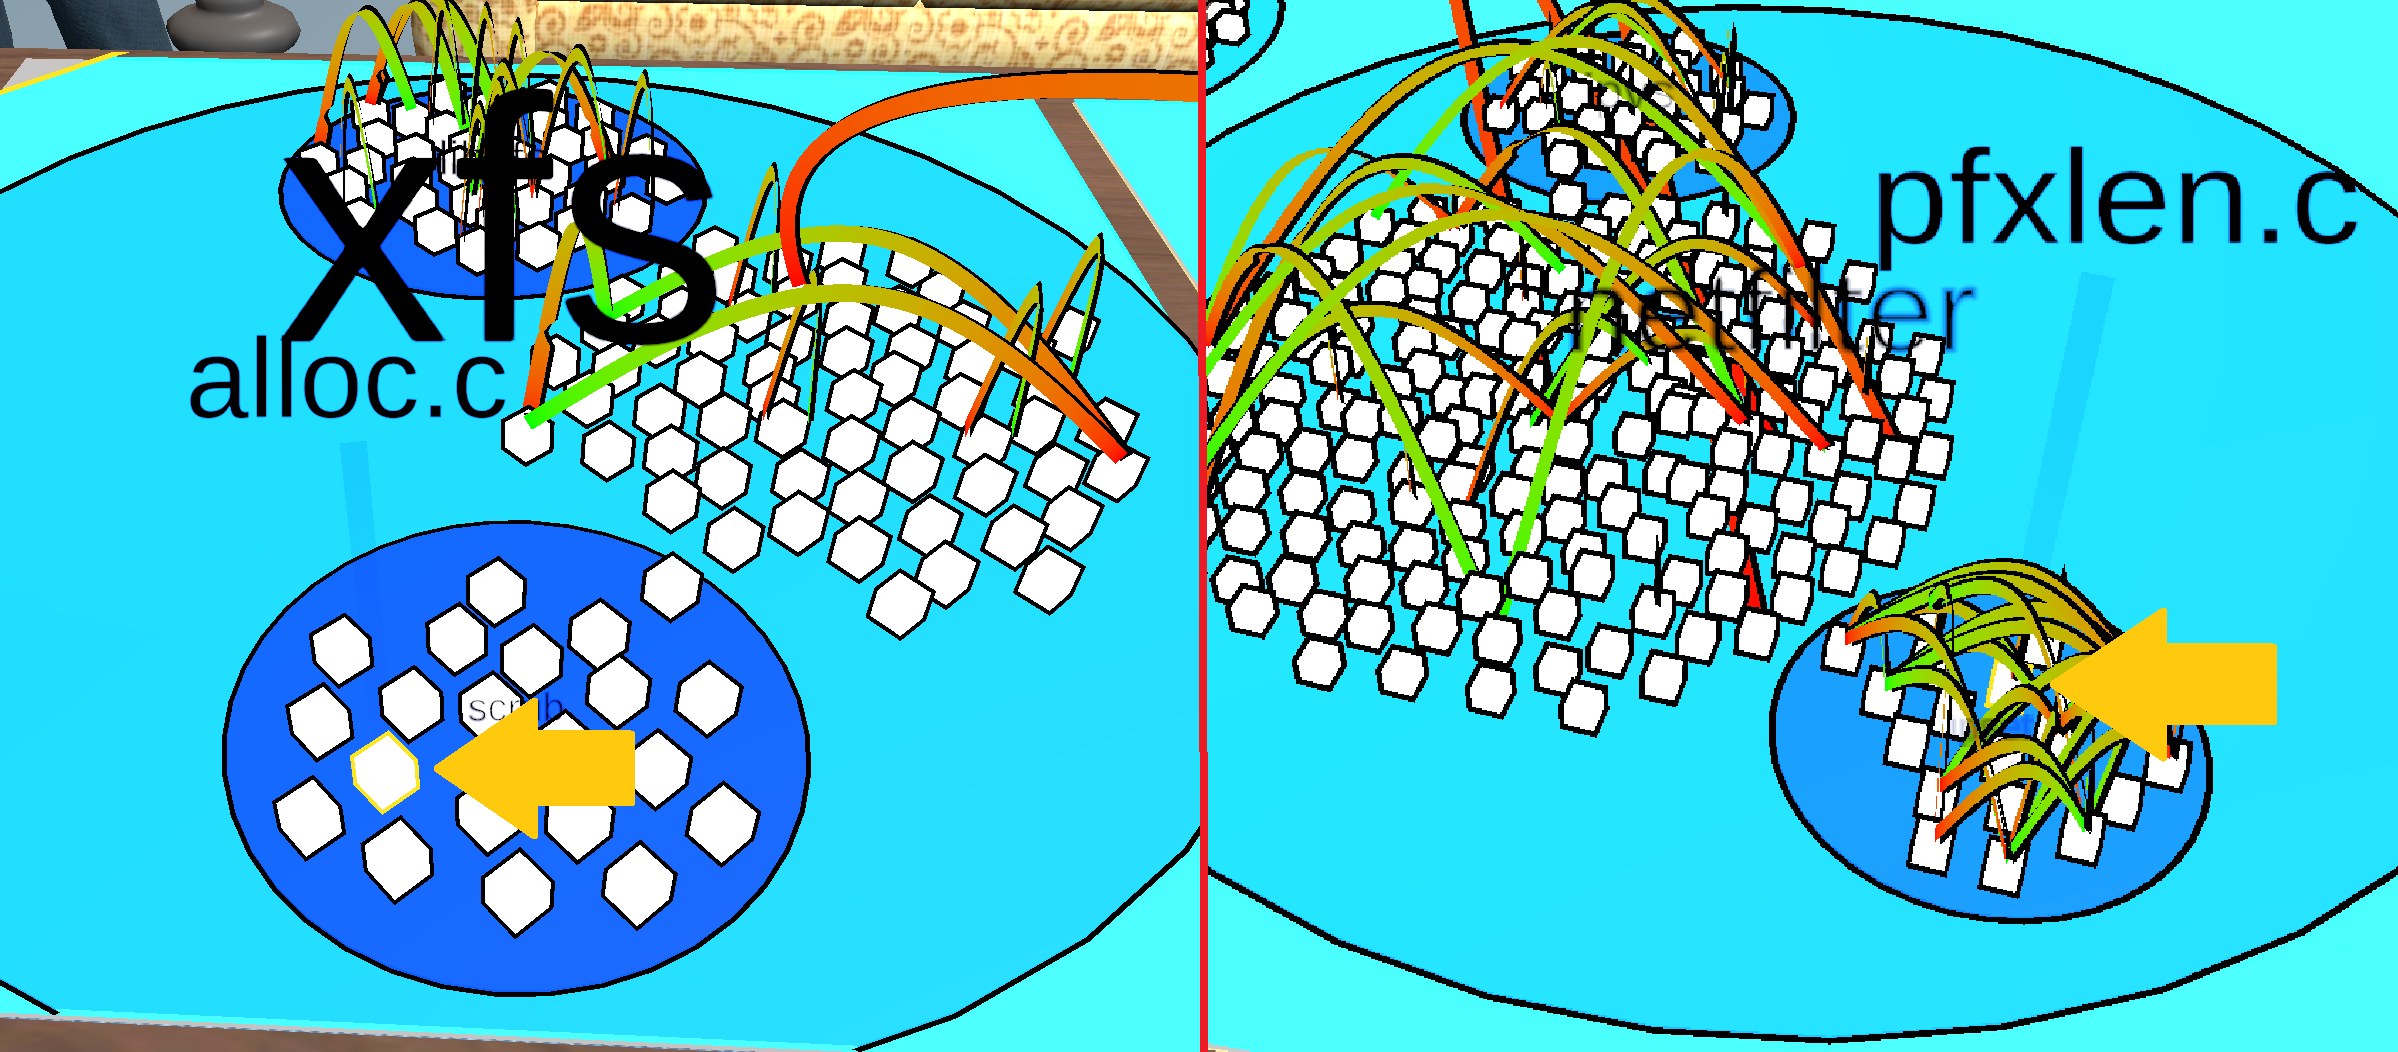
\includegraphics[width=1\textwidth]{Evaluation/img/task1.png}
    \caption{The two key nodes are marked with a yellow arrow}\label{fig:task1}
\end{figure}
\subsubsection{Execution}